\section{Introduction}
\paragraph*{}
Image edges are locations of sharp change of brightness, i.e. locations of high local contrast. As a consequence of being a contrast-based feature, the presence and position of an edge is not altered by global illumination changes in the image; which contributes to the robustness of Edge Detection-based solutions.

\paragraph*{}
Edge detection techniques come in two variants depicted in \reffig{1D2DEdges}. \textbf{1D~Edge Detection} methods scan the image along a path and locate the points of intersection between image edges and the scan line. \textbf{2D~Edge Detection} methods locate the entire edge. In this chapter we will inspect the first technique, featuring remarkable performance and sub-pixel precision.

\twoFigures
{img/1DEdgeDetection/edge1D}
{img/1DEdgeDetection/edge2D}
{\textbf{1D Edge Detection}, \textbf{2D Edge Detection}}
{1D2DEdges}
{\basicWidth}

\paragraph*{}
We will start with a short description of the methodology of extracting a 1D image brightness profile along a given path and then proceed to detection of the features present in the profile.

\paragraph*{}
Depending on the nature of the brightness change that constitutes an edge, we distinguish two kinds of edges: \textbf{step edges}, occurring between two areas of different intensity, and \textbf{ridge edges} (or simply ridges), occurring where image intensity changes briefly and then returns to initial value.

\paragraph*{}
A wide class of visual inspection tasks is focused on the areas bounded by two step edges of opposite polarity, rather than on the edges considered separately. Because of that it is useful to consider such areas as a third, additional type of feature discernible in one-dimensional profile; here called a \textbf{stripe}.  

\paragraph*{}
Overall, the chapter will cover detection of three kinds of features discernible in 1D profiles, all demonstrated in \reftab{1DFeatures}. In each example the feature (step edge, ridge or stripe) is vertical and the image is scanned horizontally to find the points of intersection between the feature and the scan line.

\begin{table}[h]
\centering
\begin{tabular}{c c c}
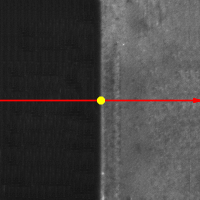
\includegraphics[width=0.275\textwidth]{img/1DEdgeDetection/edge}
& 
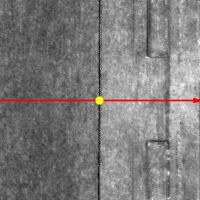
\includegraphics[width=0.275\textwidth]{img/1DEdgeDetection/ridge}
&
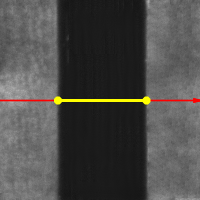
\includegraphics[width=0.275\textwidth]{img/1DEdgeDetection/stripe}
\\
\textbf{Step Edge} &
\textbf{Ridge} &
\textbf{Stripe} 
\end{tabular}
\caption{Different kinds of image features extracted from 1D profile.}
\label{tab:1DFeatures}
\end{table}